\chapter{Conceituação Teórica}\label{cap2}


A popularidade dos computares permite a criação e compartilhamento de textos onde a quantidade de informação facilmente extrapola a capacidade de humana de leitura e análise de coleções de documentos, estejam eles disponíveis na Internet ou em computadores pessoais. A necessidade de simplificar e organizar grandes coleções de documentos criou uma demanda por modelos de aprendizado de máquina para extração de conhecimento em bases textuais. Para esse fim, foram desenvolvidas técnicas para descobrir, extrair e agrupar textos de grandes coleções, entre essas, a modelagem de tópicos~\cite{Hofmann1999,Deerwester1990,Lee1999,Blei2012}.  %--> não falar só de modelagem de tópicos. Falar de RI com referências



% -> Recuperação de Informação
\section{Recuperação de Informação}

% Necessidade de encontrar informação

Devido à popularização dos computadores e à grande disponibilidade de documentos em formato digital, em especial na Web a área da Recuperação de Informação (RI) tem recebido atenção de pesquisadores nas últimas décadas.
% 
Recuperação de informação é área da computação que envolve a aplicação de métodos computacionais no tratamento e busca de informação em bases de dados não estruturados, usualmente grandes coleções de documentos textuais armazenados em dispositivos eletrônicos.
% Tratamento == Classificação e Agrupamento?
A tarefa central da recuperação de informação é encontrar informações de interesse dos usuários e exibi-las. A principal ferramenta empregada nesse problema é o desenvolvimento de sistemas de recuperação de informação (SRI). Nesses sistemas o usuário expressa sua necessidade por meio da formulação de uma consulta, usualmente composta por um conjunto de palavras-chave. Então, o sistema apresenta os resultados da busca, frequentemente documentos, em ordem de relevância com a consulta.



\subsection{Modelos de Recuperação de Informação}

Um modelo de recuperação de informação deve criar representações de documentos e consultas a fim de predizer a necessidade expressa nos termos da consulta. Com base na entrada do usuário esses modelos buscam por documentos similares aos termos da consulta. Segue abaixo a descrição dos três modelos clássicos para recuperação de informação.

\subsubsection{Modelo Booleano}

O modelo booleano ou modelo lógico foi um dos primeiros modelos aplicados a recuperação informação sendo utilizado a partir de 1960. Nesse modelo uma consulta é considerada uma sequencia de termos conectador por operadores lógicos como AND, OR e NOT. Como resultado, classifica cada documento como relevante ou não relevante à consulta, sem gradação de relevância. Esse operadores lógicos poder ser manipulados por usuários com algum conhecimento em álgebra booleana para aumentar a quantidade de resultados ou restringi-la.

Esse modelo apresenta como principal desvantagem a impossibilidade de ordenação dos resultados por relevância, uma vez que para muitos sistemas de RI o \textit{ranking} dos resultados é uma característica essencial, principalmente em grades bases de dados. 

As vantagens desse modelo são a facilidade de implementação e a possibilidade de usuários experientes usarem os operadores lógicos como uma forma de controle sobre os resultados da busca. Por outro lado, para usuários inexperientes isso pode ser considerado uma desvantagem, uma vez que o uso expressões lógicas não é intuitivo. Apesar dos problemas apresentados, visto sua simplicidade, esse modelo foi largamente utilizado em sistemas comerciais. 



\subsubsection{Modelo Vetorial}


Uma das formas mais comuns para representação textual é conhecida como Modelo Espaço Vetorial (\textit{Vectorial Space Model} - VSM)~\cite{Rezende2003}, onde os documentos e consultas são representados como vetores em um espaço Euclidiano $t$-dimensional em que cada termo extraído da coleção é representado por uma dimensão. 
% 
Considera-se que um documento pode ser representado pelo seu conjunto de termos, onde cada termo $k_i$ de um documento $d_j$ associa-se um peso $w_{ij}\geq0$ que indica a importância desse termo no documento. 
%
De forma similar, para uma consulta $q$, associa-se um peso $w_{i,q}$ ao par termo consulta que representa a similaridade entre a necessidade do usuário e o termo $k_i$. 
%
Assim o vetor associado ao documento $d_j$ é dado por $\vec{d}_{j} = (w_{1,j}, w_{2,j}, ..., w_{t,j})$. 
%
De forma similar, o vetor associado a consulta $q$ é dado por $\vec{q} = (w_{1,q}, w_{2,q}, ..., w_{t,q})$.


No modelo vetorial, a similidade entre um documento $d_j$ e uma consulta $q$ é calculada pela correlação entre os vetores $\vec{d_j}$ e $\vec{q}$, a qual pode ser medida pelo cosseno do  ângulo entre esses vetores, conforme mostrado na Equação~\ref{equ:cosseno-doc-consulta}.



\begin{equation}
sim(d_j, q) = \frac{ \vec{d_j} \bullet \vec{q} }
                   { |\vec{d_j}| \times | \vec{q}|}
            = \frac{ \sum_{i=1}^{t} w_{i,j} \cdot w_{i,q} }
                   { \sqrt{\sum_{i=1}^{t} w_{i,j}^2} \times \sqrt{\sum_{i=1}^{t} w_{i,q}^2 } }                   \label{equ:cosseno-doc-consulta}		                   
\end{equation} 


Valores de cosseno próximos a 0 indicam um ângulo próximo a 90º entre $\vec{d_j}$ e $\vec{q}$, ou seja, o documento $d_j$ compartilha poucos termos com a consulta $q$, enquanto valores próximos a 1 indicam um ângulo próximo a 0º, ou seja, $d_j$ e $q$ compartilham termos e são similares~\cite{Tan2005,Feldman2006}.

Avaliar a relevância de um documento sob uma consulta é fundamental para os modelos de RI. Para isso pode-se utilizar medidas estatísticas simples como a frequência do termo, conhecida como TF (do inglês \textit{Term Frequency}) e a frequência de documentos, conhecida como DF (do inglês \textit{Document Frequency}). A frequência do termo indica o número de vezes que um termo ocorre na coleção de documentos. A frequência de documentos, indica o número de documentos que contém ao menos uma ocorrência de um determinado termo. Considera-se que os termos que ocorrem frequentemente em muitos documentos, em geral, não trazem informações úteis para discriminar a relevância dos documentos, então, a fim de diminuir o peso de termos altamente frequentes, usa-se o fator IDF (\textit{Inverted Document Frequency}), que é o inverso da número de documentos que contem um termo. O IDF é a medida de informação que um termo fornece com base em quão raro ou comum esse termo é para a coleção. Seja $N$ o número de documentos de uma coleção e $n_i$ o número de documentos onde o termo $k_i$ ocorre, o cálculo de IDF é dado por: 

	\begin{equation}
		IDF(k_i) = log\frac{N}{n_i}
		\label{equ:IDF}
	\end{equation}

Entre a medidas mais populares para ranqueamento de buscas está a TF-IDF (\textit{Term Frequency-Inverted Document Frequency}) que pondera a frequência de um termo em um documento com sua frequência na coleção total de documentos. Assim, a relevância de um termo para um documento é dada por:

\begin{equation}
	w_{i,j} = freq_{i,j} \cdot IDF(k_i)
\end{equation}



Onde $freq_{i,j}$ é a frequência do termo $k_i$ no documento $d_j$. A medida TF-IDF atribui valores altos para termos que ocorrem frequentemente em um documentos, e valores menores para termos que ocorrem poucas vezes em um documento ou em muitos documentos da coleção. A ideia da medida tf.idf e quantificar a importância de um termo em um documento com base em sua frequência no próprio documento e sua distribuição ao longo da coleção de documentos~\cite{Croft2009,Salton1988,Shamsinejadbabki2012,Salton:1994}.


Uma vez que o sistema calcula os graus de similaridade entre os documentos e a busca por meio da equação~\ref{equ:cosseno-doc-consulta}, é possível ranquear os resultados por ordem de relevância. Além disso, sua relativa simplicidade e flexibilidade, favorecem a aplicação desse modelo em sistemas de recuperação de informação
~\cite{Tan2005,Croft2009,Manning2008}.

% ->-----------------------------------------------------------------------


\subsubsection{Modelo Probabilístico}

 
O modelo probabilístico é baseado no princípio da ordenação probabilística (\textit{Probability Ranking Principle}) onde dada um consulta q e um documento $d_j$ relevante a $q$, o modelo tenta estimar a probabilidade do usuário encontrar o documento $d_j$. O modelo assumente que para uma consulta $q$ há um conjunto de documentos $R$ que contém exatamente os documentos relevantes e nenhum outro, sendo este um conjunto resposta ideal que maximiza a probabilidade do usuário encontrar um documento $d_j$ relevante a $q$. 

Seja $\overline{R_q}$ o complemento de $R$ de forma que $\overline{R_q}$ contém todos os documentos não relevantes à consulta $q$. Seja $P(R_q|d_j)$ a probabilidade do documento $d_j$ ser relevante à consulta $q$ e $P(\overline{R_q}|d_j)$ a probabilidade de $d_j$ não ser relevante à $q$. A similaridade entre um documento $d_j$ e uma consulta $q$ é definida por:


\begin{equation}
	sim(d_j, q) = \frac{P(R_q|dj)}{P(\overline{R_q}|dj)}
\end{equation}


% -> Explicar o (odds ratio)



% -> Segmentação 

\documentclass{sig-alternate-05-2015}
\usepackage[portuguese]{babel}
%\usepackage{multirow}
%\usepackage{adjustbox}
%\usepackage{graphicx}
%\usepackage{array}
%\usepackage{tabulary}
% \usepackage{pgfplotstable}
% recommended:
%\usepackage{booktabs}
%\usepackage{array}
%\usepackage{colortbl}
%\usepackage{emptypage}
%\newcolumntype{l}[1]{>{\centering\arraybackslash}p{#1}}
% \usepackage{showframe}   %% just for demo
% \usepackage[brazilian,hyperpageref]{backref}	 % Paginas com as citações na bibl
% \usepackage[alf]{abntex2cite}	% Citações padrão ABNT
\usepackage[utf8]{inputenc}		% Codificacao do documento (conversão automática dos acentos)

\usepackage{rotating}
\usepackage{tabularx}
\usepackage{multicol}
\usepackage{amsmath}
\usepackage[linesnumbered,ruled]{algorithm2e}




% Define o caminho das figuras
\graphicspath{{images/}}



\begin{document}

\title{Segmentação topical automática de atas de reunião}


\numberofauthors{1} 

\author{
\alignauthor Ovídio José Francisco\\
       \email{ovidiojf@gmail.com}
}

\maketitle

%\begin{abstract}   
%
%\end{abstract}

\section*{RESUMO}



\keywords{}

\begingroup
\let\clearpage\relax

\section{Introdução}
	\label{sec:introducao}
	Frequentemente atas de reunião tem a característica de apresentar um texto com poucas quebras de parágrafo e sem marcações de estrutura, como capítulos, seções ou quaisquer indicações sobre o tema do texto. 


% Definição 

A tarefa de segmentação textual consiste dividir um texto em partes que contenham um significado relativamente independente. Em outras palavras, é identificar as posições onde há uma mudança significativa de tópicos.

% Usos
É útil em aplicações que trabalham com textos sem quebras de assunto, ou seja, não apresentam parágrafos, seções ou capítulos, como transcrições automáticas de áudio e grandes documentos que contêm assuntos não idênticos como atas de reunião e noticias.


% Interesses
O interesse por segmentação textual tem crescido em em aplicações voltadas a recuperação de informação %citar o [15] ...
e sumarização de textos. % ... e [2] do "Efficient Linear T S"
Essa técnica pode ser usada para aprimorar o acessao a informação quando essa é solicitada por um usário por meio de uma consulta, onde é possível oferecer porções menores de texto mais relevante ao invés de exibir um documento maior que pode conter informações menos pertinente. A sumarização de texto também pode ser aprimorada ao processar segmentos separados por tópicos ao invés de documentos inteiros.


% Coesão Léxica
Os algoritmos avaliados baseiam-se na ideia de coesão léxica entre assuntos. Isto é, a mudança de tópicos é acompanhada % é relacionada à
 de uma proporcional mudança de vocabulário. A partir disso, vários algorítmos foram propostos. Nesse artigo, os principais serão analizados na prespectiva de atas de reunião.





% Diversas aplicações fazem uso de segmentação textual, incluindo 

% Entre as principais mais frequentes de segmentação textual estão a tra



%É principalmente utilizada em aplicações que processam textos longos como transcrições de áudio e documentos longos, além de aprimorar técnicas de sumarização e information retrievel.



% Usos:
%	* quando não há identificações
%	* em transcrições de áudio
%	* em documentos longos
% 	* text summarization (ver a referencia [2] de Efficient Linear Text...)




%Isto é, dado um texto, identificar onde há mudança de tópicos.


% Interest in automatic text segmentation has blossomed over the last few years, with applications ranging from information retrieval to text summariza-tion to story segmentation of video feeds. [A Critique and Improvement of an Evaluation Metric for Text Segmentation]



%Em outras palavras é identificar divisões entre unidade de informação sucessivas

%A tarefa de segmentação textual consiste em encontrar pontos onde há mudança de tópicos no texto.



%[ The task of linear text segmentation is to split a large text document into shorter fragments, usually blocks of consecutive sentences. ]


% **Segmentação é identificar divisiões entre unidades de informação sucessivas (Beeferman, Berger, and Lafferty (1997))**

%   [Text segmentation is the task of determining the positions at which topics change in a stream of text]






\section{Trabalhos Relacionados}
	\label{sec:trabalhos}
	\section{Trabalhos Relacionados}
	\label{sec:trabalhos}


Semelhante a esse trabalho, outras abordagens foram propostas como em~\cite{CHAIBI2014} onde os autores adaptam os \textit{TextTiling} e \textit{C99} ao idioma árabe. Apresentam os resultados de experimentos no qual avaliam a performance em jornais de diferentes países em árabe. As adaptações consistem basicamente na etapa de pré-processamento e apontam que diferenças no dialeto de cada pais devem ser consideradas no processo de segmentação e que a adaptação depende da escolha de um \textit{stemmer} adequado.

É recorrente a aplicação de segmentadores à reuniões com múltiplos participantes onde se estuda os discursos extraídos de reuniões, ou seja, o texto a ser segmentado é uma transcrição das falas dos participantes durante a reunião.
%
Banerjee~\cite{Banerjee2006} apresenta um segmentador baseado no  \textit{TextTiling} ao contexto das reuniões, com múltiplos participantes. Utiliza como \textit{corpus} a transcrição da fala dos participantes durante a reunião a qual foi conduzida por um mediador que propunha os tópicos e anotava o tempo onde os participantes mudavam o assunto. 
% outros exemplos são

Ainda no contexto de reuniões com múltiplos participantes, alguns elementos da fala são utilizados para encontrar melhores segmentos.
%
Bokaei~\cite{Bokaei2015}, traz um trabalho voltado à segmentação funcional do texto, que foca na atividade dos participantes, as quais categoriza em diálogos e monólogos e sugere que alguns comportamentos podem dar pistas de mudança de tópico, como quando um participante toma a palavra por um tempo prolongado. 
Galley~\cite{Galley2003} por sua vez considera de elementos como pausas, trocas de falantes e entonação para encontrar melhores segmentos.

Kern aponta em sua pesquisa~\cite{Kern2009} que algoritmos que apresentam melhor performance o fazem ao custo de maior complexidade computacional, que se deve à construção de matrizes de similaridade entre todas as sentenças como em~\cite{Choi2000}. Ele apresenta uma abordagem que otimiza o cálculo ao computar as médias das similaridades de cada bloco, a qual chama de \textit{inner similarity} e em seguida usa esses valores para calcular as medias das similaridades entre todos os blocos a qual chama de \textit{outter similarity}. Dessa forma não é criada uma matriz que contem as similaridades de todas as sentenças, mas apenas daquelas mais próximas. Os autores reportam uma eficiência superior e uma eficiência comparável aos algoritmos mais complexos.
% usa vetores contendo o peso da palavra ao inves da frequencia.




\section{Adaptação às atas de reunião}
	\label{sec:adaptacaoasatas}
	\section{Proposta: Segmentação Linear Automática de Atas de Reunião}
	\label{sec:proposta}






%%%%%%%%%%
% TextTiling e C99 criados para inglês e independente de domínio
%%%%%%%%%%
Os algoritmos \textit{TextTiling} e \textit{C99} foram propostos para o inglês, independentemente de domínio, ou seja, a proposta inicial dos autores é trabalhar em qualquer texto nessa língua.
%%%%%%%%%%
% Adapatar para Atas em português
%%%%%%%%%%
Assim, propõe-se adaptá-los ao contexto das atas de reunião em português do Brasil, ou seja, em uma língua diferente e dentro de um contexto específico. As subseções seguintes tratam das adaptações para esse nicho mais específico. A Seção~\ref{sec:avaliacao} mostra a análise dos algoritmos adaptados.

%%%%%%%%%%
% Dificuldade: Coesão léxica não tão bem definida
%%%%%%%%%%
O vocabulário das reuniões, ainda que em tópicos diferentes, compartilham certo vocabulário pertencente ao ambiente onde se deram as reuniões. Isso é um fator que diminui a coesão léxica entre os segmentos.
%%%%%%%%%%
% Dificuldade: estilo da escrita
% - Paragrafo único
% - Cabeçalhos e rodapés
% - Pontuação --> ; encerrando sentenças
% - Insersão de espaços que não são quebra de sentença
% - Ruídos
%%%%%%%%%%
As atas de reunião costumam ter um estilo de escrita que deve ser levado em conta na adaptação do algoritmos, como a identificação de finais de sentença na ausência de quebras de parágrafo, inserção de linhas que não separam assuntos, utilização de pontuação para transição de tópicos, e cabeçalhos e numerais ruidosos. 

Nas subseções a seguir serão apresentados o pré-processamento e a identificação de segmentos candidatos considerados para a segmentação de atas.





\subsection{Pré-processamento}
	\label{subsec:preprocessamento}




	O texto a ser segmentado frequentemente é extraído de documentos em formatos como \textit{pdf}, \textit{doc}, \textit{docx} ou \textit{odt}. Após a extração do texto, esse pode passar por processos de transformação os quais serão apresentados a seguir.
	
%	A etapa de pré-processamento, em um documento contendo texto puro, acontece em quatro passos principais. 

  \begin{figure}[!h]
	\centering
	
\includegraphics[width=0.2\textwidth]{construcao.png}
%	\caption{Exemplo de pré-processamento.}
	\\Em Construção
	\label{fig:exemplopreprocessamento}
  \end{figure}

	
%\begin{enumerate}


%
% 1) Identificação de sentenças
%\item \textit{Identificação de sentenças}: 
%Cada final de sentença e identificado e marcado com uma \textit{string} especial, esse processo é melhor descrito na Subseção~\ref{subsec:indentificacaosentencas}.
%
%conforme mostrado no Algoritmo~\ref{alg:identificacaofinaisdesent}.

%	
% 2) Eliminação de ruídos
%\item \textit{Remoção de ruídos}:

%%%%%%%%%%
% Cabeçalhos e rodapés
%%%%%%%%%%
%As atas frequentemente contém trechos que podem ser considerados pouco informativos e descartados durante o pré-processamento, como cabeçalhos e rodapés que se misturam aos tópicos tratados na reunião, podendo ser  inseridos no meio de um tópico e criando uma quebra que prejudica tanto o algoritmo de segmentação, quanto a leitura do texto pelo usuário.
%%%%%%%%%%
% Numerais
%%%%%%%%%%
%Também é comum o uso de numerais para marcação de páginas e linhas, da mesma forma, são pouco informativos e podem ser descartados.


%%%%%%%%%%
% Remoção de ruídos
%%%%%%%%%%
%Nesse trabalho, esses elementos são removidos, uma vez que, o descarte não causa perca de informação e pode facilitar a identificação dos segmentos, pois melhora a coesão do texto. Outro benefício é manter o texto livre de trechos que fogem do assunto circundante.
%%%
% TODO: Como são removidos?
% por meio de heurísticas simples
%%%

%Elimina-se também nesse passo a acentuação, sinais de pontuação, restando apenas palavras.  



%	
% 3) Stop Words
%\item \textit{Stop Words}: 
%Remove-se as palavras consideradas menos informativas, as quais são chamadas de \textit{stop words}, para isso, utiliza-se uma lista contendo 438 palavras. 

%
% 4) Stemming
%\item \textit{Stemming}:
%Extrai-se o radical de cada palavra, para isso, as letras são convertidas em caixa baixa e aplica-se o algoritmo \textit{Orengo}\footnote{\urlorengo} para remoção de sufixos.


%\end{enumerate}
	
	



%Tem-se então, uma lista com os elementos considerados mais significativos do texto. %A Figura~\ref{fig:exemplopreprocessamento} mostra a etapa de pré-processamento em uma sentença em português.
	



%  \begin{figure}[!h]
%	\centering
%	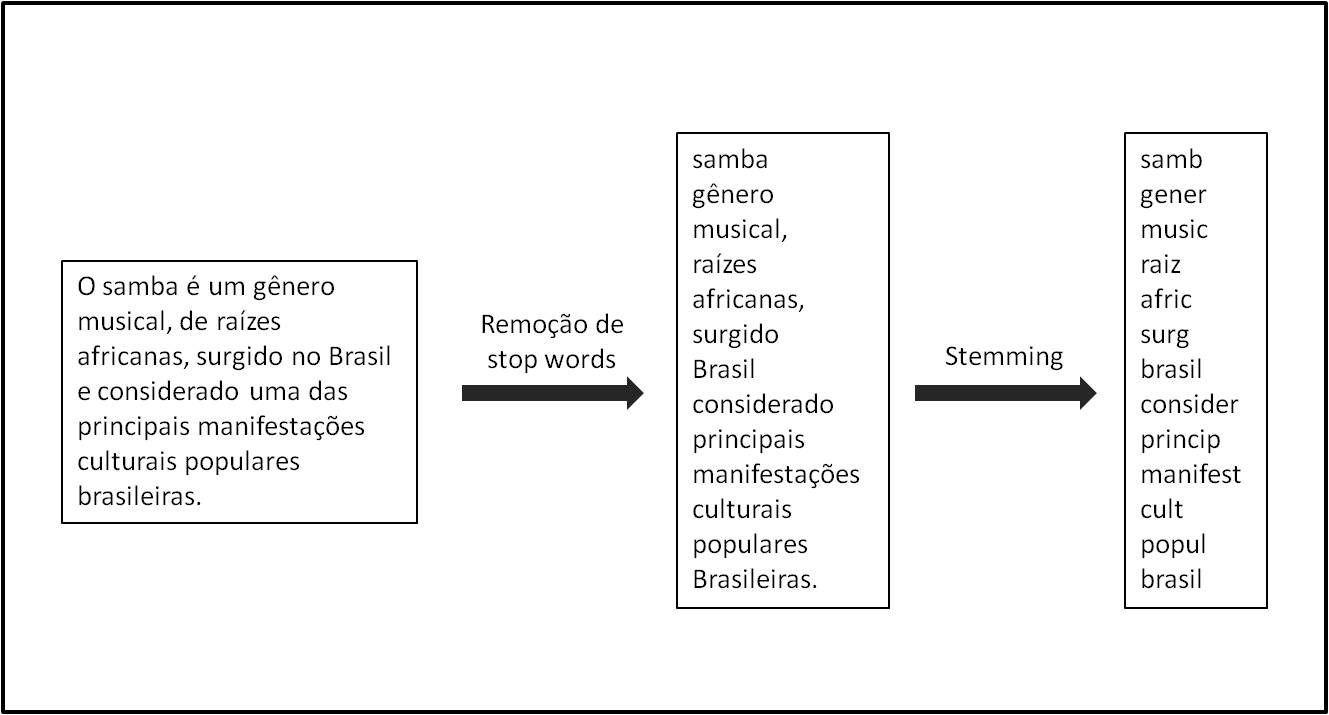
\includegraphics[width=0.45\textwidth]{exemplo-preprocessamento.jpg}
%	\caption{Exemplo de pré-processamento.}
%	\label{fig:exemplopreprocessamento}
%  \end{figure}






\subsection{Identificação de candidatos}
	\label{subsec:indentificacaosentencas}
	
%%%%%%%%%%	
% Indicar unidade mínima de Segmento
%%%%%%%%%%
	
	
%	Como entrada para os 
%	Os algoritmos de segmentação devem ser
	É preciso fornecer aos algoritmos os candidatos iniciais a limites de segmento. Para isso, é necessário escolher qual será a unidade de informação mínima que constitui um segmento. Baseando-se no estilo de escrita e considerando as pontuações de um texto, é possível, em alguns casos, indicar quebras de parágrafo, finais de sentenças ou mesmo palavras como elementos que encerram um segmento. 

	Ocorre que em atas de reunião é uma prática comum redigi-las de forma que o conteúdo discutido fica em parágrafo único, além disso, as quebras de parágrafo são usados para formatação de outros elementos como espaço para assinaturas. 
%
	Também não é conveniente indicar todo ponto entre \textit{token} como candidato pois obrigaria a ajustar posteriormente os segmentos de maneira a não quebrar uma ideia ou frase. 
%	
	Assim, neste trabalho, os finais de sentença são considerados unidades de informação e portanto, passíveis a limite entre segmentos. 
	
	Devido ao estilo de pontuação desses documentos, como encerrar sentenças usando um \textit{";"} e inserção de linhas extras, foram usadas as regras apresentadas no Algoritmo 1 para identificar os finais de sentenças.  


\begin{algorithm}
	\SetKwInOut{Input}{Entrada}
	\SetKwInOut{Output}{Saída}
	\SetKwBlock{Inicio}{início}{fim}
	\SetKwFor{ParaTodo}{para todo}{}{fim para todo}
	\SetKwIF{Se}{SenaoSe}{Senao}{}{}{senao se}{senao}{fim se}
	\SetKwFor{Para}{}{}{}
%	\SetKwAlgorithm{Algorithm}{Algoritmo}{}

	
	\Input{Texto}
	\Output{Texto com identificações de finais de sentença}
	
	\ParaTodo {token, marcá-lo como final de sentença se:} {	

	Terminar com um \texttt{!}\\
	Terminar com um \texttt{.} e não for uma abreviação\\
	Terminar em \texttt{.?;} e:
		\Para{}{
			For seguido de uma quebra de parágrafo ou tabulação\\
			O próximo \textit{token} iniciar com  \texttt{(\{["'}\\
			O próximo \textit{token} iniciar com letra maiúscula\\
			O penúltimo caracter  for \texttt{)\}]"'}\\
		}
	}
	
	\caption{Identificação de finais de sentença}
	\label{alg:identificacaofinaisdesent}
\end{algorithm}









%Como forma de padronização, as instituições acrescentam ao documento

%		passos menores
%		1 - heurística simples para remover cabeçalho e rodapé.
%		2 - remoção de numerais
%		3 - remoção de acentos, transformações de caixa, remoção de pontuação.
		
	% Esses passos são realizados internamente em cada algorímo, para que a saida seja legível ao usuário final.





%A qualidade do algoritmo é sempre dependente da escrita correta! Ausência de emoticons, códigos de computador e gírias.





%Nas subseções a seguir serão expostas as alterações para aumentar a eficiência dos algoritmos e encontrar o melhor modelo para a tarefa de segmentar o texto das atas em tópicos.



%Tais aspectos não se aplicam ao contexto das atas, onde o estilo de escrita em forma de narrativa, prefere poupar o leitor de diálogos secundários durante transições de tópicos. 







	
	
%Elimina-se textos considerados de pouca relevância como a numeração de páginas e linhas, cabeçalhos e rodapés, também elemina-se acentuação, sinais de pontuação, restando apenas palavras.  


	
	
%%
%% 1) Identificação de sentenças
%Primeiro cada final de sentença e identificado e marcado com uma \textit{string} especial, esse processo é melhor descrito na Subseção~\ref{subsec:indentificacaosentencas}.
%%
%%conforme mostrado no Algoritmo~\ref{alg:identificacaofinaisdesent}.
%
%%	
%% 2) Eliminação de ruídos
%Depois, elimina-se textos considerados de pouca relevância como a numeração de páginas e linhas, cabeçalhos e rodapés, também elemina-se acentuação, sinais de pontuação, restando apenas palavras.  
%
%%	
%% 3) Stop Words
%Em seguida, remove-se as palavras consideradas menos informativas, as quais são chamadas de \textit{stop words}, para isso, utiliza-se uma lista contendo 438 palavras. 
%
%%
%% 4) Stemming
%Por fim, extrai-se o radical de cada palavra, para isso, as letras são convertidas em caixa baixa e aplica-se o algoritmo \textit{Orengo}\footnote{\urlorengo} para remoção de sufixos.
%
%
%Tem-se então, uma lista com os elementos considerados mais significativos do texto. A Figura~\ref{fig:exemplopreprocessamento} mostra a etapa de pré-processamento em uma sentença em português.
%	





	

\section{Avaliação}
	\label{sec:avaliacao}
	
\section{Avaliação}
	\label{sec:avaliacao}



%%%%%%%%%% 
% Necessidade de uma referência
%%%%%%%%%%
Para que se possa avaliar um segmentador automático de textos, é preciso uma referência, isto é, um texto com os limites entre os segmento conhecidos. Essa referência, deve ser confiável, sendo uma segmentação legítima que é capaz de dividir o texto em porções relativamente independentes, mantendo um conteúdo legível, ou seja, uma segmentação ideal.
%

Entre as abordagens mais comuns para se conseguir essas referências, encontramos: A concatenação aleatória de documentos distintos, onde o ponto entre o final de um texto e o inicio do seguinte é um limite entre eles. A segmentação manual dos documentos, nesse caso, pessoas capacitadas, também chamadas de juízes, ou mesmo o autor do texto, são consultadas e indicam manualmente onde há uma quebra de segmento. Em transcrição de conversas faladas em reuniões com múltiplos participantes, um mediador é responsável por encerrar um assunto e iniciar um novo, nesse caso o mediador anota manualmente o tempo onde há uma transição de tópico. Em aplicações onde a segmentação é tarefa secundária, analisar seu impacto na aplicação final.


%%%%%%%%%%
% As 2 principais dificuldades na avaliação
%%%%%%%%%%
De acordo com \cite{Pevzner2002} há duas principais dificuldades na avaliação de segmentadores automáticos. A primeira é conseguir um referência, já que juízes humanos costumam não concordar entre si, sobre onde os limites estão e outras abordagens podem não se aplicar ao contexto. A segunda é que tipos diferentes de erros devem ter pesos diferentes de acordo com a aplicação. Há casos onde certa imprecisão é tolerável e outras, como a segmentação de notícias, onde a precisão é mais importante.


%%%%%%%%%%
% Definição do que é um bom algoritmo de segmentação
%%%%%%%%%%
Para fins de avaliação desse trabalho, um bom método de segmentação é aquele cujo resultado melhor se aproxima do ideal, sem a obrigatoriedade de estar perfeitamente alinhado com tal. Ou seja, visto o contexto das atas de reunião, e a subjetividade da tarefa, não é necessário que os limites entre os segmentos (real e hipótese) sejam idênticos, mas que se assemelhem em localização e quantidade.


Para quantificar a eficiência dos algoritmos, segue uma revisão das principais métricas aplicáveis.

As próximas subseções mostram o conjunto de atas e a segmentação usada como referência, uma revisão das principais métricas aplicáveis à segmentação e os testes realizados a fim de avaliar os métodos

\subsection{Conjunto de documentos}
	A fim de obter um conjunto de documentos segmentados que possam servir como referência na avaliação, seis atas de reunião foram coletadas junto ao departamento de computação da UFSCar-Sorocaba. Os documentos foram oferecidos à profissionais que participam de reuniões desse departamento e por meio de um \textit{software} segmentaram o texto das atas conforme o julgamento de cada um. Os segmentos gerados manualmente foram comparados à segmentação automática conforme os critérios descritos a seguir.
	
	As atas de reunião diferem dos textos comumente estudados em outros trabalho em alguns pontos.
	


\subsection{Medidas de Avaliação}


	As medidas de avaliação tradicionalmente utilizadas em \textit{information retrieval} como precisão e revocação trazem alguns problemas na avalização de segmentadores automáticos.  
Conforme o algoritmo aponta mais segmentos no texto, tende a melhorar a revocação e ao mesmo tempo, reduzir a precisão, um problema que pode ser contornado usando \textit{F-measure} que faz uma combinação da duas levando em conta seus pesos, o que por outro lado é mais difícil de interpretar. 
Essas medidas falham ao não serem sensíveis a \textit{near misses}, ou seja, quando um limite não coincide exatamente com o esperado, mas fica próximo~\cite{Kern2009}.

A Figura~\ref{fig:exemplosegmentacaozoom} mostra um exemplo com duas segmentações hipotéticas e uma referência. Em ambos os casos não há nenhum verdadeiro positivo, o que implica em zero para os valores de precisão, acurácia, e revocação, embora a segunda hipótese possa ser considerada superior à primeira se levado em conta a proximidade dos limites.



  \begin{figure}[!h]

	\centering
	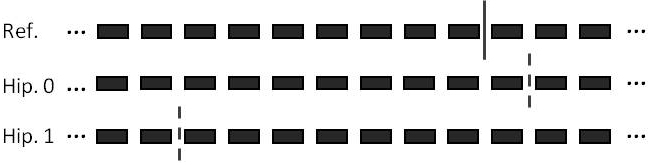
\includegraphics[width=0.47\textwidth]{windiffzoom.jpg}
	\caption{Exmplos de segmentação}
	\label{fig:exemplosegmentacaozoom}

  \end{figure}



\subsubsection{P$_k$}
A fim de resolver o problema de \textit{near misses}, Beeferman \textit{et. al.}~\cite{Beeferman1999} apresentam uma nova medida chama P$_k$ que atribui valores parciais a \textit{near misses}. Esse método move uma janela de tamanho $k$ e a cada posição e verifica se o início e o final da janela estão ou não dentro do mesmo segmento e penaliza o algoritmo em caso de discrepância. 

Ou seja, dado duas palavras de distancia $k$, uma discrepância é computada quando o algoritmo e a referência não concordam se as palavras estão ou não no mesmo segmento.

O valor de $k$ é calculado como a metade da média dos comprimentos dos segmentos reais. Como resultado, é retornado a contagem de discrepâncias divido pelo quantidade de segmentações analisadas. Esse valor serve como medida de dissimilaridade entre as segmentações e pode ser interpretada como a probabilidade de duas sentenças extraídas aleatoriamente pertencerem ao mesmo segmento.



\subsubsection{WindowDiff}

Pevzner~\cite{Pevzner2002} aponta problemas na avaliação mais tradicional Pk~\cite{Beeferman1999}. Eles apontam que esse método penaliza demasiadamente os falsos negativos em relação aos falsos positivos e a \textit{near misses}, além disso, desconsidera o tamanho e a quantidade de segmentos, entre outros problemas.

Como solução, propõem um novo método, o qual chamam de \textit{WindowDiff} que traz duas diferenças principais: a dobra a penalidade para os falsos positivos a fim de diminuir o problema da subestimação dessa medida e, diferente de P$_k$, ao mover a janela pelo texto, penaliza o algoritmo sempre que o número de limites proposto pelo algoritmo não coincidir com o número de limites esperados para aquela janela de texto. 

Com isso, demonstram em seu trabalho que, em relação a P$_k$, consegue resolver seus principais problemas e mantém sua proposta inicial de sensibilidade a \textit{near misses}, penalizando-os menos que os falsos positivos puros.


  \begin{figure}[!h]

	\centering
	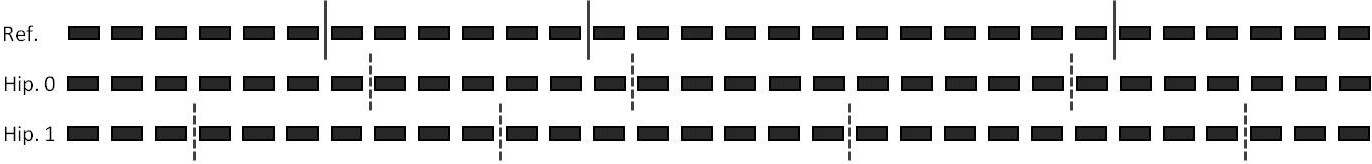
\includegraphics[width=0.47\textwidth]{windiff.jpg}
	\caption{Exemplo de construção de uma matriz de rank}
	\label{fig:exemplosegmentacao}

  \end{figure}
  
  

%Falar do software para segmentação manual????


\subsection{Avaliação dos segmentadores}


%%%%%%%%%%
% Parâmetros
%%%%%%%%%%
As implementações dos algoritmos permitem ao usuário a configuração de seus parâmetros. 
%
O \textit{TextTiling} permite ajustarmos dois parâmetros, sendo, o tamanho da janela (distância entre a primeira e a última sentença) para o qual atribuiu-se os valores 20, 40 e 60. O segundo parâmetro, o passo (distância que a janela desliza), atribuiu-se os valores 3, 6, 9 e 12. Gerando ao final 18 modelos.
%

O \textit{C99} permite ajustarmos três parâmetros, sendo, a quantidade segmentos desejados, o qual é calculado como uma proporção dos candidatos a limite. Para isso atribuiu-se as proporções de 0,2 a 1,0 em intervalos de 0,2 O segundo parâmetro, o tamanho da máscara utilizada para gerar a matriz de ranking, atribuiu-se os valores 9 e 11. Permite ainda, definirmos se as sentenças serão representados por vetores contendo a frequência ou o peso de cada termo, onde ambas as representações foram utilizadas. Gerando ao final 20 modelos.



%%%%%%%%%%
% Cálculo das medidas para cada modelo
%%%%%%%%%%
Pela comparação dos resultados com a segmentação fornecida pelos especialistas, calculou-se para cada modelo as medidas tradicionais acurácia, precisão, revocação, F-medida. Além dessas, computou-se também as métricas mais aplicadas à segmentação textual P$_k$ e \textit{WindowDiff}.



%%%%%%%%%%
% Teste de Fiedman e CD
% 1ª Etapa
%%%%%%%%%%
Em seguida aplicou-se o teste de Friedman a fim de saber se há diferenças significativas entre a eficácia dos modelos, o pós-teste de Nemenyi foi aplicado para descobrir quais diferenças são significativas. 
%
Exite diferença quando seus \textit{rankings} médios diferirem em um valor mínimo, chamado de diferença critica (CD). 
%

%%%%%%%%%%
% Dados Obtidos
%%%%%%%%%%
Com isso foi possível, pela análise do diagrama de diferença crítica, verificar qual é o melhor modelo para cada medida
% e quão significativamente 
em relação aos demais. 


A tabela~\ref{tab:mediasC99} mostra os dados obtidos com o \textit{C99}, onde \texttt{S} é a proporção de segmentos em relação a quantidade de candidatos, \texttt{M} é o tamanho da máscara utilizada para criar a matriz de \textit{ranking} e \texttt{W} indica se os segmentos são representados por vetores contendo a frequência ou um peso das palavras. 



\begin{table}[!h]
	\centering

	\begin{tabular}{|c|c|c|c|c|}
	
		\hline
		Medida & \texttt{S} & \texttt{M} & \texttt{W} & \textbf{Média}\\		
		\hline

		Acuracy		& 40	& 11 & Sim & 0.6199	\\ \hline	
		F1			& 60	& 9	 & Sim & 0.6167	\\ \hline	
		Precision	& 40	& 11 & Sim & 0.7106	\\ \hline			
		Recall		& 100	& 9	 & Não & 0.8516	\\ \hline		
		Pk			& 40	& 11 & Sim & 0.1163	\\ \hline	
		Windiff		& 40	& 11 & Sim & 0.3800	\\ \hline		

		
	\end{tabular}
	
	\caption{Médias das medidas obtidas com \textit{C99}}
	\label{tab:mediasC99}
\end{table}


A tabelas~\ref{tab:mediasTextTiling} mostra os dados obtidos com o \textit{TextTiling}, \texttt{J} é o tamanho da janela e \texttt{P} e o passo.

\begin{table}[!h]
	\centering

	\begin{tabular}{|c|c|c|c|}
	
		\hline
		Medida & \texttt{J} & \texttt{P} & \textbf{Média}\\		
		\hline

		Acuracy		& 50 & 9 	& 0.5510 \\ \hline	
		F1			& 50 & 3 	& 0.5898 \\ \hline	
		Precision	& 60 & 12 	& 0.5746 \\ \hline			
		Recall		& 50 & 3 	& 0.7717 \\ \hline		
		Pk			& 30 & 9 	& 0.1572 \\ \hline	
		Windiff		& 50 & 9 	& 0.4489 \\ \hline		

		
	\end{tabular}
	
	\caption{Médias das medidas obtidas com o \textit{TextTiling}}
	\label{tab:mediasTextTiling}
\end{table}


Uma vez sabendo quais valores de parâmetros melhor configuram um algoritmo para uma medida, resta então saber qual dos dois algoritmos é mais eficiente segundo essa medida. Para isso aplicou-se novamente o teste de Friedman com pós-teste de Nemenyi, dessa vez, com os melhores modelos dos dois algoritmos para cada medida. O resultado segue na Tabela~\ref{tab:melhoresmodelos}

\begin{table}[!h]
	\centering
	
	\begin{tabular}{|c|c|c|c|c|}

		\hline
		Medida & Algoritmo & \texttt{S} & \texttt{M} & \texttt{W}\\		
		\hline
		
	
		Acuracy		& C99 & 40 	& 11	& Sim \\ \hline
		Precision	& C99 & 40 	& 11	& Sim \\ \hline
		Pk			& C99 & 40 	& 11	& Sim \\ \hline
		Windiff		& C99 & 40 	& 11	& Sim \\ \hline
		F1			& C99 & 60 	& 9		& Sim \\ \hline
		Recall		& C99 & 100 & 9		& Não \\ \hline
 	
	
	\end{tabular}

	\caption{Melhores modelos para cada medida segundo diagramas de diferença crítica}
	\label{tab:melhoresmodelos}	
	
\end{table}


Na análise do diagrama de diferença crítica verificou-se que o algoritmo \textit{C99} apresenta melhor eficiência em todas as medidas e os valores das quatro primeiras os valores de \texttt{S}, \texttt{M} e \texttt{W} se repetiram, sugerindo uma configuração otimizada para o problema da segmentação de atas de reunião.







	
\section{Análise dos Resultados}
	\label{sec:resultados}
	\section{Resultados}
	\label{sec:resultados}

%%%%%%%%%%
% Objetivos
%%%%%%%%%%
A fim de encontrar o melhor método que divida uma ata em segmentos coerentes, realizou-se experimentos com o \textit{TextTiling} e \textit{C99} a fim de encontrar os melhores parâmetros para esses documentos.

%tópicos retornando segmentos  que retorne segmentos coerentes 

%%%%%%%%%%
% Parâmetros
%%%%%%%%%%
As implementações dos algoritmos permitem ao usuário a configuração de seus parâmetros. 
%
O \textit{TextTiling} permite ajustarmos dois parâmetros, sendo, o tamanho da janela (distância entre a primeira e a última sentença) para o qual atribuiu-se os valores 20, 40 e 60. Para o segundo parâmetro, o passo (distância que a janela desliza), atribuiu-se os valores 3, 6, 9 e 12. Gerando ao final 20 modelos.
%

O \textit{C99} permite ajustarmos três parâmetros, sendo, a quantidade segmentos desejados, o qual é calculado como uma proporção dos candidatos a limite. Para isso atribuiu-se as proporções {0,2; 0,4; 0,6; 0,8; 1,0}. O segundo parâmetro, o tamanho da máscara utilizada para gerar a matriz de ranking, atribuiu-se os valores 9 e 11. Permite ainda, definirmos se as sentenças serão representados por vetores contendo a frequência ou o peso de cada termo, onde ambas as representações foram utilizadas.
%
 Considerando todos os parâmetros, foram gerados 20 modelos para o algoritmo C99.% By Rafael 



%%%%%%%%%%
% Cálculo das medidas para cada modelo
%%%%%%%%%%

% --> Isso já foi falado no texto
%Pela comparação dos resultados com a segmentação fornecida pelos especialistas, calculou-se para cada modelo as medidas tradicionais acurácia, precisão, revocação, F-medida. Além dessas, computou-se também as métricas mais aplicadas à segmentação textual P$_k$ e \textit{WindowDiff}.



%%%%%%%%%%
% Teste de Fiedman e CD
% 1ª Etapa
%%%%%%%%%%
Em seguida aplicou-se o teste de Friedman a fim de saber se há diferenças significativas entre a eficácia dos modelos. O pós-teste de Nemenyi foi aplicado para descobrir quais diferenças são significativas. 
%
Exite diferença quando seus \textit{rankings} médios diferirem em um valor mínimo, chamado de diferença critica (CD). 
%

%%%%%%%%%%
% Dados Obtidos
%%%%%%%%%%
Com isso foi possível, pela análise do diagrama de diferença crítica, verificar qual é o melhor modelo para cada medida
% e quão significativamente 
em relação aos demais. 


A Tabela~\ref{tab:mediasC99} mostra os dados obtidos com o \textit{C99}, onde \texttt{S} é a proporção de segmentos em relação a quantidade de candidatos, \texttt{M} é o tamanho da máscara utilizada para criar a matriz de \textit{ranking} e \texttt{W} indica se os segmentos são representados por vetores contendo a frequência ou um peso das palavras. 



\begin{table}[!h]
	\centering

	\begin{tabular}{|c|c|c|c|c|}
	
		\hline
		Medida & \texttt{S} & \texttt{M} & \texttt{W} & \textbf{Média}\\		
		\hline

		Acuracy		& 40	& 11 & Sim & 0.6199	\\ \hline	
		F1			& 60	& 9	 & Sim & 0.6167	\\ \hline	
		Precision	& 40	& 11 & Sim & 0.7106	\\ \hline			
		Recall		& 100	& 9	 & Não & 0.8516	\\ \hline		
		Pk			& 40	& 11 & Sim & 0.1163	\\ \hline	
		Windiff		& 40	& 11 & Sim & 0.3800	\\ \hline		

		
	\end{tabular}
	
	\caption{Médias das medidas obtidas com \textit{C99}}
	\label{tab:mediasC99}
\end{table}


A tabelas~\ref{tab:mediasTextTiling} mostra os dados obtidos com o \textit{TextTiling}, onde \texttt{J} é o tamanho da janela e \texttt{P} é o passo.

\begin{table}[!h]
	\centering

	\begin{tabular}{|c|c|c|c|}
	
		\hline
		Medida & \texttt{J} & \texttt{P} & \textbf{Média}\\		
		\hline

		Acuracy		& 50 & 9 	& 0.5510 \\ \hline	
		F1			& 50 & 3 	& 0.5898 \\ \hline	
		Precision	& 60 & 12 	& 0.5746 \\ \hline			
		Recall		& 50 & 3 	& 0.7717 \\ \hline		
		Pk			& 30 & 9 	& 0.1572 \\ \hline	
		Windiff		& 50 & 9 	& 0.4489 \\ \hline		

		
	\end{tabular}
	
	\caption{Médias das medidas obtidas com o \textit{TextTiling}.}
	\label{tab:mediasTextTiling}
\end{table}


Uma vez sabendo quais valores de parâmetros melhor configuram um algoritmo para uma medida, resta então saber qual dos dois algoritmos é mais eficiente segundo essa medida. Para isso aplicou-se novamente o teste de Friedman com pós-teste de Nemenyi, dessa vez, com os melhores modelos dos dois algoritmos para cada medida. O resultado segue na Tabela~\ref{tab:melhoresmodelos}

\begin{table}[!h]
	\centering
	
	\begin{tabular}{|c|c|c|c|c|}

		\hline
		Medida & Algoritmo & \texttt{S} & \texttt{M} & \texttt{W}\\		
		\hline
		
	
		Acuracy		& C99 & 40 	& 11	& Sim \\ \hline
		Precision	& C99 & 40 	& 11	& Sim \\ \hline
		Pk			& C99 & 40 	& 11	& Sim \\ \hline
		Windiff		& C99 & 40 	& 11	& Sim \\ \hline
		F1			& C99 & 60 	& 9		& Sim \\ \hline
		Recall		& C99 & 100 & 9		& Não \\ \hline
 	
	
	\end{tabular}

	\caption{Melhores modelos para cada medida segundo diagramas de diferença crítica.}
	\label{tab:melhoresmodelos}	
	
\end{table}


Na análise do diagrama de diferença crítica verificou-se que o algoritmo \textit{C99} apresenta melhor eficiência em todas as medidas e os valores das quatro primeiras os valores de \texttt{S}, \texttt{M} e \texttt{W} se repetiram, sugerindo uma configuração otimizada para o problema da segmentação de atas de reunião.






	
\section{Conclusão}
	\label{sec:conclusao}
	\section{Conclus�o}
	\label{sec:conclusao}

As atas de reuni�o, objeto de estudo desse artigo, apresentam caracter�sticas peculiares em rela��o � discursos e textos em geral. Caracter�sticas como segmentos curtos e coes�o mais fraca devida ao estilo que evita repeti��o de palavras e ideias em benef�cio da leitura por humanos, dificultam o processamento por computadores.

%%%%%%%%%%
% Benef�cios 
%%%%%%%%%%


Os algoritmos \textit{TextTiling} e \textit{C99} foram testados em um conjunto de atas coletadas do Departamento de Computa��o da UFSCar-Sorocaba. Por meio da an�lise dos dados chegou-se a uma configura��o cujos segmentos melhor se aproximaram das amostras segmentadas por participantes das reuni�es. 


Na maioria das medidas, o algoritmo \textit{C99} sobressaiu-se em rela��o ao \textit{TextTiling}, contudo, os testes estat�sticos, n�o apresentam diferen�a significativa. 


%%%%%%%%%%%%%%%
% O Impacto do Preprocessamento 
%%%%%%%%%%%%%%%

Da mesma forma, a etapa de preprocessamento proporciona melhora de performance quando aplicada, por�m o seu maior benef�cio � a diminui��o do custo computacional, uma vez que n�o prejudica a qualidade dos resultados.



A segmenta��o de atas de reuni�o pode ajudar na organiza��o, busca e compreens�o dos conte�dos nelas contidos. Tamb�m outros dom�nios e aplica��es diferentes podem se beneficiar dos resultados apresentados, como aplica��es voltadas a resgate de informa��o, sumariza��o e acessibilidade. Assim, espera-se que outros trabalhos possam aproveitar deste.
	
	
Em trabalhos futuros, ser�o investigadas t�cnicas de extra��o de t�picos para descrever os segmentos e com isso aprimorar o acesso ao conte�do das atas de reuni�o.





\endgroup



\bibliographystyle{abbrv}
\bibliography{sigproc}  % sigproc.bib is the name of the Bibliography in this case
	
\pagestyle{empty}
 	\label{sec:anexo}
 	\include{project/anexo}
\end{document}


% -> Representação

\section{Representação de Textos} \label{subsection:RepTextos}

As etapas anteriores produzem fragmentos de documentos onde o texto esta em um estágio de processamento inicial, com menos atributos que as versões originais, onde cada fragmento está associado a um tema, porém, ainda desestruturado. Ocorre que as técnicas de mineração de texto exigem uma representação estruturada dos textos conforme será visto na Seção~\ref{subsection:RepTextos}.

Uma das formas mais comuns para que a grande maioria dos algoritmos de aprendizado de máquina possa extrair padrões das coleções de textos é a representação no formato matricial conhecido como Modelo Espaço Vetorial (\textit{Vectorial Space Model} - VSM)~\cite{Rezende2003}, onde os documentos são representados como vetores em um espaço Euclidiano $t$-dimensional em que cada termo extraído da coleção é representado por um dimensão. Assim, cada componente de um vetor expressa a relação entre os documentos e as palavras. Essa estrutura é conhecida como \textit{document-term matrix} ou matriz documento-termo. Uma das formas mais populares para representação de textos é conhecida como \textit{Bag Of Words} a qual é detalhada a seguir.
	
%\subsubsection{Espaço Vetorial} \cite{Rezende2003}

%\subsubsection{Extração de Termos}

\subsection{\textit{Bag Of Words}} \label{subsubsec:BOW}
Após a etapa de pré-processamento, onde as \textit{stop words} foram removidas e as palavras reduzidas ao seus radicais (\textit{stemming}), tem-se uma versão reduzida, com menos atributos, dos dados originais. Essa versão pode ser facilmente convertida em uma tabela ou matriz documento-termo. Essa representação, conhecida como \textit{bag-of-words}, onde cada palavra (termo) não eliminada é transformado em um atributo (\textit{feature})~\cite{Rezende2003}.	Essa representação é mostrada pela Tabela \ref{table:bagofwords}.
		

\begin{table}[!h]
	\centering

	\begin{tabular}{c|c|c|c|c|c|c|c}


	& $Term_1$ & \dots & \dots & $Term_k$ & \dots & \dots & $Term_n$ \\ \hline \hline
	$d_1$ & $a_{11}$ & \dots & \dots & $a_{1k}$ & \dots & \dots & $a_{1n}$   \\ \hline 
	\dots & \dots    & \dots & \dots & \dots    & \dots & \dots & \dots      \\ \hline 
	$d_j$ & $a_{j1}$ & \dots & \dots & $a_{jk}$ & \dots & \dots & $a_{jn}$   \\ \hline 
	\dots & \dots    & \dots & \dots & \dots    & \dots & \dots & \dots      \\ \hline 
	$d_m$ & $a_{m1}$ & \dots & \dots & $a_{mk}$ & \dots & \dots & $a_{mn}$   \\ 

	\end{tabular}
	\caption{Coleção de documentos na representação \textit{bag-of-words}}
	\label{table:bagofwords}\\ 
\end{table}



Essa forma de representação sintetiza a base de documentos em um contêiner de palavras, ignorando a ordem em que ocorrem, bem como pontuações e outros detalhes, preservando apenas o peso de determinada palavra nos documentos.	É uma simplificação de toda diversidade de informações contidas na base de documentos sem o propósito de ser uma representação fiel do documento, mas oferecer a relação entre as palavras e os documentos a qual é suficiente para a maioria dos métodos de aprendizado de máquina~\cite{Rezende2003}. 
%https://en.wikipedia.org/wiki/Document-term_matrix

%=====================
%Sumarizaç\~ao????
%Como Calcular a Avaliaç~ao? Precis~ao? Recall????
%=======================

%\subsubsection{Métricas de relevância dos termos} 

Após a extração dos termos, esses devem receber pesos de acordo com sua relevância dentro da base de documentos. As medidas mais tradicionais são a binária, onde o termo recebe o valor 1 se ocorre em determinado documento ou 0 caso contrário; \textit{document frequency}, é o número de documentos no qual um termo ocorre; \textit{term frequency - tf}, atribui-se ao peso a frequência do termo dentro de um determinado documento; \textit{term frequency-inverse document frequency, tf-idf}, pondera a frequência do termo pelo inverso do número de documentos da coleção em que o termo ocorre.

% (Manning et al., 2008; Feldman e Sanger, 2006) Tese Rafael		



% -> Extração de Tópicos
\section{Modelos de Extração de Tópicos}

% Na venda do peixe, citar que a busca é tão difícil quanto a leitura e análise de coleções de documentos.

Os modelos de extração de tópicos são abordagens não-supervisionadas que visam descobrir padrões latentes nas relações entre os documentos e seus termos.  Baseiam-se na premissa de que um documento é produzido a partir de tópicos previamente definidos que determinam os termos a serem utilizados em um documento. Nesse contexto, um documento é uma mistura de tópicos onde cada termo presente no documento pode ser associado a um tópico. Um tópico por sua vez, é uma estrutura com valor semântico que representada por um conjunto de termos e seus pesos que indicam o quão significante esses termos são para um assunto e pode ser útil para o entendimento do tema ao qual o tópico trata.

Para descobrir esses tópicos, algumas técnicas foram propostas. Em termos de metodologia, a maioria dos trabalho enquadram-se em duas principais categorias, os modelos não-probabilísticos e os modelos probabilísticos.


% -- \subsection{Modelos Não Probabilísticos}

Os modelos não-probabilísticas baseiam-se em técnicas de fatoração de matrizes, onde a matrix documento-termo é projetada em um espaço com menor dimensionalidade chamado \textit{Latent Semantic Space}. 
Seja
$d \in D = \{d_1,\cdots,d_n\}$ o vetor que representa a coleção de documentos, 
$t \in T = \{t_1,\cdots,t_m\}$ seus termos distintos e 
$z \in Z = \{z_1,\cdots,z_k\}$ seus tópicos. 
Esses métodos aprendem decompondo a matriz documento-termo $W$, em duas matrizes $Z$ e $A$, tal que a resultante de $ZA$ seja uma aproximação da matriz $W$ original. Mais formalmente tem-se:

\begin{equation}
	Z\cdot A = \hat{W} \approx W
\end{equation}

A matriz $A$ corresponde a matriz documento-tópico e possui dimensão $k \times n$. $Z$ corresponde a matriz termo-tópico e possui dimensão $m \times k$ onde $n$ é o número de termos, $m$ é o número de documentos da coleção e $k$ é a quantidade de tópicos a serem extraídos. Uma vez que $k \ll n,m$, então $A$ e $Z$ são menores que a matriz de entrada, o que resulta em uma versão comprimida da matriz original, pois $k \cdot n + m \cdot k \ll n \cdot m$. Ao final, obtém-se uma representação documento-tópico que atribui um peso para cada tópico em cada documento da coleção e uma representação termo-tópico que representa a probabilidade de ocorrência de um termo em um documento dado que o tópico está presente no documento.

 Nesse sentido, o \textit{Latente Semantic Indexing} (LSI) usa a técnica chamada \textit{Singular Value Decomposition} (SVD) para encontrar padrões no relacionamento entre assuntos e termos em uma coleção de texto não estruturada. Entretanto, esse método não fornece uma interpretação para elementos com valores negativos~\cite{Deerwester1990}~\cite{Cheng2013}. % Trocar essa referência do Cheng2013 pela que ele usa na seção 2 do trabalho dele.

% -- NMF
Outro modelo popular é o \textit{Non-Negative Matrix Factorization} (NMF).  Diferente do LSI, no processo de fatoração apenas operações aditivas são permitidas, o que garante que as matrizes resultantes não possuem elementos negativos, permitindo uma interpretação mais intuitiva de seus valores. Além disso, o processo de fatoração proporciona a propriedade de \textit{clustering}, ou seja, agrupar as colunas da matriz $W$, e dessa forma, oferece a característica interessante de agrupar os documentos da coleção.  % -< Onde é utilizado


% -- \subsection{Modelos Probabilísticos}

Os modelos probabilísticos consideram os documentos como uma mistura de tópicos e um tópico como uma distribuição probabilística sobre os termos. O processo de elaboração do documento a partir desses tópicos é chamado de processo generativo ou modelo generativo, o qual é desconhecido porém pode ser estimado com base nos termos presentes no documento, também chamados de variáveis observáveis. Assim, o processo de extração de tópicos consiste em estimar o modelo generativo que deu origem ao documento.
% falar em algum ponto sobre o problema das matrizes esparsas. Principalmente com documentos pequenos
% 
% -- PLSA
O PLSA foi um dos primeiros a estender o modelo LSA e formalizar a extração de tópicos probabilísticos. De maneira similar ao LSA, o esse modelo decompõe uma matriz esparsa a fim de reduzir a dimensionalidade. O PLSA cria um modelo estatístico chamado \textit{aspect model} que associa os tópicos as variáveis observáveis atribuindo probabilidades às ligações entre os tópicos e os documentos e entre as palavras e os tópicos. Assim, cada documento pode ser representado como a probabilidade de um tópico estar presente, $P(z|d)$. E a probabilidade de um termo ocorrer dado que um tópico esta presente, $P(t|z)$. Em comparação ao LSA, é considerado uma método mais robusto por proporcionar uma interpretação probabilística. Por outro lado, esse modelo apresenta desvantagens como o número de parâmetros do modelo que cresce linearmente com o número de documentos da coleção que pode ocasionar \textit{overfitting}.   % - E o Expectation Maximization?

% -- LDA
A fim de contornar esses problemas, o LDA estende o modelo PLSA incorporando um modelo generativo onde os cada tópico obedece à distribuição multivariada de \textit{Dirichlet} o que o torna menos propenso ao \textit{overfitting} e capaz de inferir tópicos a documentos ainda não observados. É referenciado na literatura como estado da arte sobre modelos probabilísticos de extração de tópicos e influencia uma grande quantidade de trabalhos, tornando-se base para novos modelos. No modelo LDA, o processo de geração de palavras se dá em duas etapas:

\begin{enumerate}
	\item Atribui-se uma distribuição aleatória sobre os tópicos.
	\item Para cada termo no documento:
		\begin{enumerate}
			\item Atribui-se aleatoriamente a um tópico da distribuição obtida na etapa 1;
			\item Seleciona-se aleatoriamente uma palavra do tópico correspondente.
		\end{enumerate}
\end{enumerate}

Assim cada documento é associado a múltiplos tópicos com proporções distintas (etapa 1). Cada palavra do documento é obtida de um tópico específico (etapa 2.b) que foi anteriormente obtido a partir da distribuição de tópicos do documento (etapa 2.a). Isso permite ao modelo LDA atribuir, para cada documento, múltiplos tópicos com proporções distintas~\cite{Blei2012}.

Os modelos de extração de tópicos foram inicialmente propostos para utilização em mineração texto onde são empregados na redução de dimensionalidade, extração de informações em textos, bem como na organização e recuperação de documentos, sendo utilizados para mensurar a relevância de um termo ou conjunto de termos para determinado assunto ou documento. Visto a popularidade nessas tarefas e flexibilidade dos modelos, logo notou-se sua utilidade em outros tipos de dados com atributos discretos como imagens, grafos e genética. 





% -->\section{Trabalhos Relacionados}
% -< O trabalho que mais se aproxima a este, e o ...

% Nessa seção são discutidos os principais trabalhos relacionados esta proposta. Na subseção ... são apresentados alguns 


